\documentclass[10pt,executivepaper]{article}
\usepackage[utf8]{inputenc}
\usepackage[spanish]{babel}
\usepackage{amsmath}
\usepackage{amsfonts}
\usepackage{amssymb}
\usepackage{graphics}
\usepackage{graphicx}
\usepackage[left=2cm,right=2cm,top=2cm,bottom=2cm]{geometry}
\usepackage{imakeidx}
\makeindex[columns=3, title=Alphabetical Index, intoc]
\usepackage{listings}
\usepackage{xcolor}
\usepackage{multicol}
\usepackage{changepage}
\usepackage{float}
\usepackage{cite}
\usepackage{url}
\usepackage{pdflscape}
\usepackage{listingsutf8}

\definecolor{codegreen}{rgb}{0,0.6,0}
\definecolor{codegray}{rgb}{0.5,0.5,0.5}
\definecolor{codepurple}{rgb}{0.58,0,0.82}
\definecolor{backcolour}{rgb}{0.95,0.95,0.92}

\lstdefinestyle{mystyle}{
    backgroundcolor=\color{backcolour},
    commentstyle=\color{codegreen},
    keywordstyle=\color{magenta},
    numberstyle=\tiny\color{codegray},
    stringstyle=\color{codepurple},
    basicstyle=\ttfamily\footnotesize,
    breakatwhitespace=false,
    breaklines=true,
    captionpos=b,
    keepspaces=true,
    numbers=left,
    numbersep=5pt,
    showspaces=false,
    showstringspaces=false,
    showtabs=false,
    tabsize=3,
    inputencoding=utf8,
    extendedchars=true,
    literate={á}{{\'a}}1 {ñ}{{\~n}}1 {é}{{\'e}}1,
}

\def\fillandplacepagenumber{%
 \par\pagestyle{empty}%
 \vbox to 0pt{\vss}\vfill
 \vbox to 0pt{\baselineskip0pt
   \hbox to\linewidth{\hss}%
   \baselineskip\footskip
   \hbox to\linewidth{%
     \hfil\thepage\hfil}\vss}}


\lstset{style=mystyle}

\title{Actividad: Respaldo y restauración de una máquina virtual en la nube}

\author{Instituto Politécnico Nacional\\Escuela Superior de Computo\\Desarrollo de Sistemas Distribuidos\\Adrian González Pardo\\4CV1\\21/01}
\date{\today}
\newcommand\tab[1][1cm]{\hspace*{#1}}

\begin{document}
% Portada
%encabezado
\begin{minipage}{0.4\textwidth}
	\begin{flushleft}
		
\includegraphics[scale = 0.05]{logoescom.png}
	\end{flushleft}
\end{minipage}
\begin{minipage}{0.51\textwidth}
	\begin{flushright}
		
\includegraphics[scale = 0.055]{logoipn.png}
	\end{flushright}
\end{minipage}
\begin{center}
	\par\vspace{0.5cm}{
	\huge\textbf{Instituto Politécnico Nacional \\*[0.20cm] Escuela Superior de Cómputo}}
\par\vspace{1cm}{
	\large\textbf{Desarrollo de Sistemas Distribuidos\\Actividad: Respaldo y restauración de una máquina virtual en la nube\\Curso impartido por el profesor: Pineda Guerrero Carlos\\Grupo: 4CV1\\21/01\\Alumno: Adrian González Pardo\\}
}
\par\vspace{1cm}{
	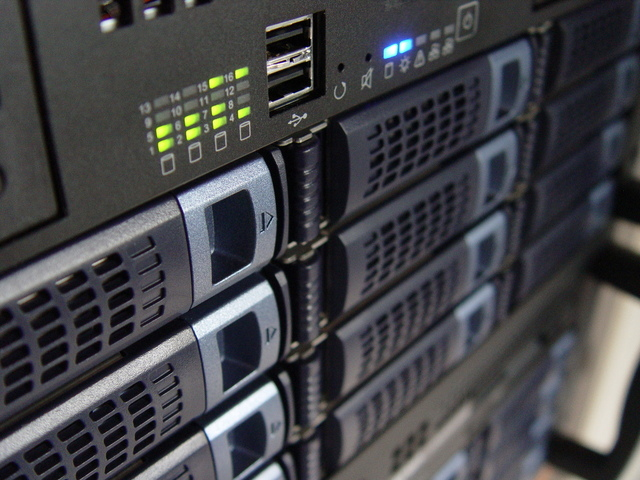
\includegraphics[scale=0.5]{servers.jpg}
}
\par\vspace{2cm}{
	Ultima fecha modificado: \today
}
\end{center}

% Indice
\clearpage
\section{Desarrollo}
Para esta practica se solicito el que ya existiera una VM creada previamente la cual puede crearse siguiendo los pasos de las practicas anteriores sin necesidad de cambiar o modificar puertos TCP, para alguna aplicación, únicamente es necesario tener la VM creada y proceder a realizar lo siguiente:
\begin{enumerate}
  \item Habilitar los respaldos de la VM
  \item Iniciar el respaldo completo
  \item Restauración de la VM
  \item Eliminación del proceso de respaldos
\end{enumerate}
\subsection{Habilitar los respaldos de la VM}
Para comenzar esta sección debemos encontrarnos en el menú de la VM con la que vamos a trabajar, con ello procederemos a lo siguiente:
\begin{center}
  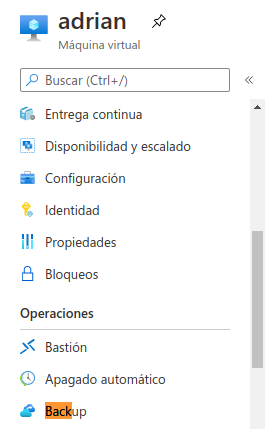
\includegraphics[scale=0.75]{imgs/1.png}\\
  \textit{Figura 1: Localización de la sección que seleccionaremos (Backup)}\\
  \clearpage
  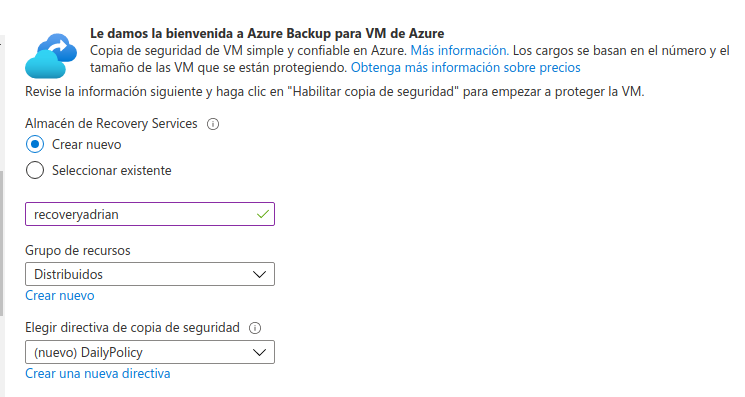
\includegraphics[scale=0.5]{imgs/2.png}\\
  \textit{Figura 2: Opciones que despliega la ventana de Backup, con ello podremos renombrar el primer campo (en este caso recoveryadrian), y con la selección predeterminada de nuestro grupo de trabajo y el tercer campo con el DailyPolicy}\\
  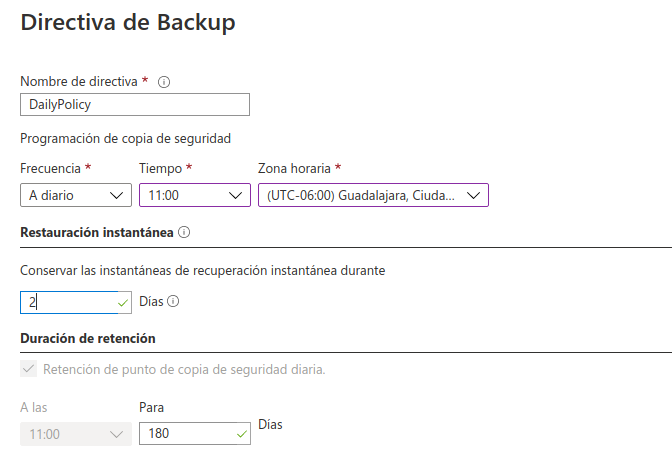
\includegraphics[scale=0.5]{imgs/3.png}\\
  \textit{Figura 3: En caso de no desear el DailyPolicy podemos crear una política con una configuración predeterminada de en que horario podemos crear los backups y con que frecuencia puede almacenarlos, y más, con ellos proderemos a implementar llendo hasta el ultimo botón de esa ventana}\\
  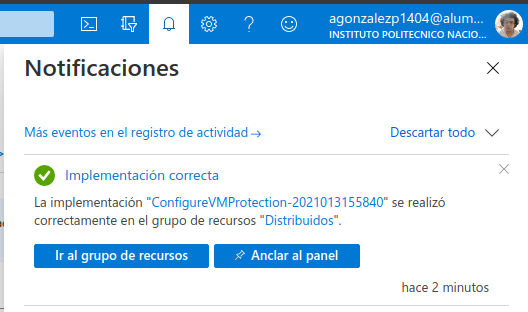
\includegraphics[scale=0.5]{imgs/4.png}\\
  \textit{Figura 4: Finalmente esperemos hasta que en el icono de la campana nos avise que nuestro backup o configuración fue implementada}
\end{center}
\subsection{Iniciar el respaldo completo}
Para comenzar esta sección debemos encontrarnos en el menú de la VM con la que vamos a trabajar, con ello procederemos a ir de nuevo al apartado de backup y tendremos lo siguiente:
\begin{center}
  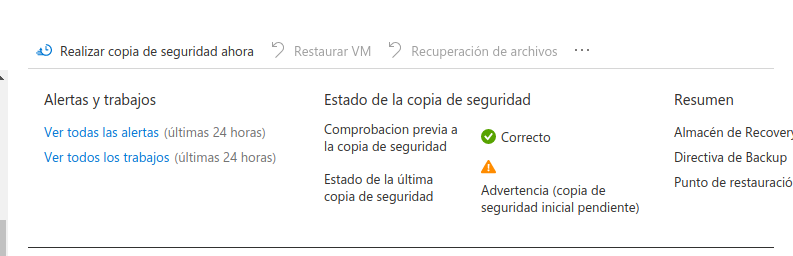
\includegraphics[scale=0.5]{imgs/5.png}\\
  \textit{Figura 5: En esta ventana inicialmente debemos ir a la parte superior que nos dice Realizar copia de seguridad ahora}\\
  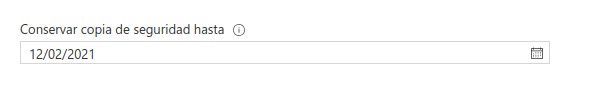
\includegraphics[scale=0.5]{imgs/6.png}\\
  \textit{Figura 6: Una vez ahi podremos o colocaremos la fecha a partir de donde se realizara el backup, para este caso se dejo el valor por default}\\
  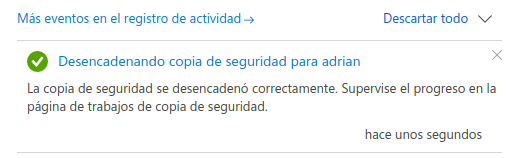
\includegraphics[scale=0.5]{imgs/7.png}\\
  \textit{Figura 7: Al igual que la figura 4 esperaremos a que se implemente nuestra configuración, y después de ello iremos a la ventana o boton que se encuentra en la Figura 5 que dice Ver todos los trabajos}\\
  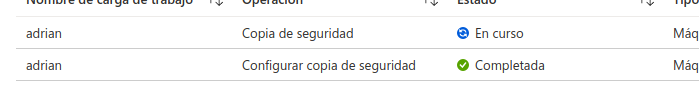
\includegraphics[scale=0.5]{imgs/8.png}\\
  \textit{Figura 8: Aquí en esta parte podremos observar el proceso de nuestro backup, y esperaremos a que concluya}\\
  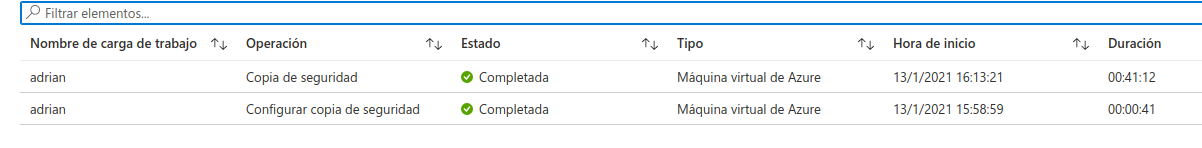
\includegraphics[scale=0.35]{imgs/9.png}\\
  \textit{Figura 9: Apartado del backup concluido (Tardo 42 minutos aproximadamente)}
\end{center}
\subsection{Restauración de la VM}
Para esta parte es necesario crear un espacio provisional de almacenamiento por ello antes de comenzar primero debemos realizar los siguiente:
\subsubsection{Creación de almacenamiento provisional}
Para ello podemos ir a nuestro portal de azure y en el buscador escribir \textit{Cuentas de almacenamiento}, en ella le daremos en crear nuevo recurso:
\begin{center}
  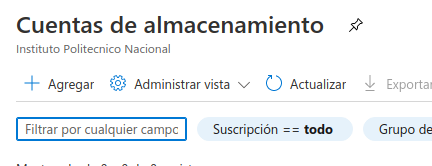
\includegraphics[scale=0.5]{imgs/ventana_cuenta.png}\\
  \textit{Figura 10: Ventana de donde crearemos el recurso}\\
  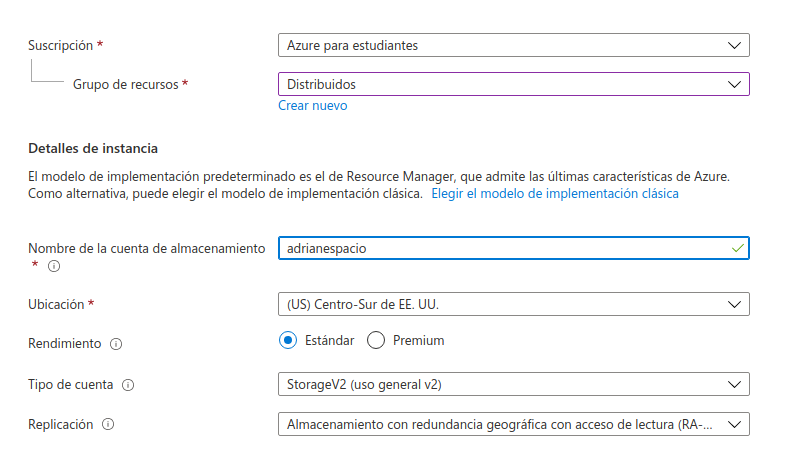
\includegraphics[scale=0.5]{imgs/almacenamiento.png}\\
  \textit{Figura 11: Campos que llenaremos para crear el recurso}\vspace{1cm}
\end{center}
Continuando para la restauración haremos lo siguiente:
\begin{center}
  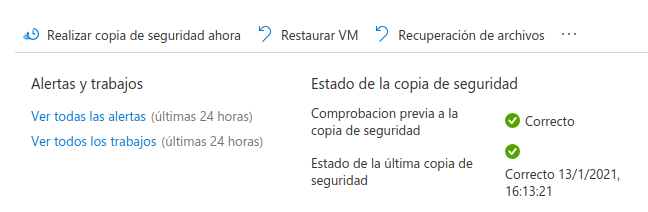
\includegraphics[scale=0.5]{imgs/10.png}\\
  \textit{Figura 12: Mismo caso que todos nuestros anteriores pasos, en Backup ir a Restaurar VM}\\
  \begin{landscape}
    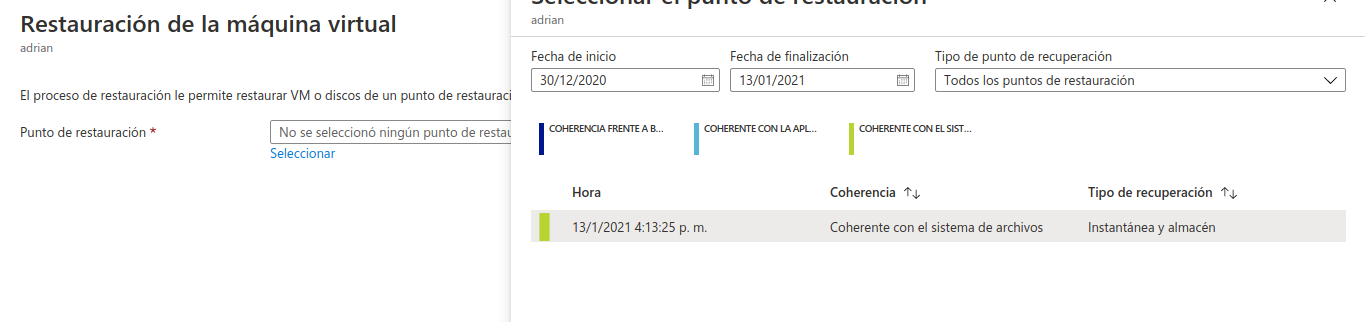
\includegraphics[scale=0.45]{imgs/11.png}\\
    \textit{Figura 13: En esta sección se fue al apartado de selección y se selecciono el ultimo backup}\\
    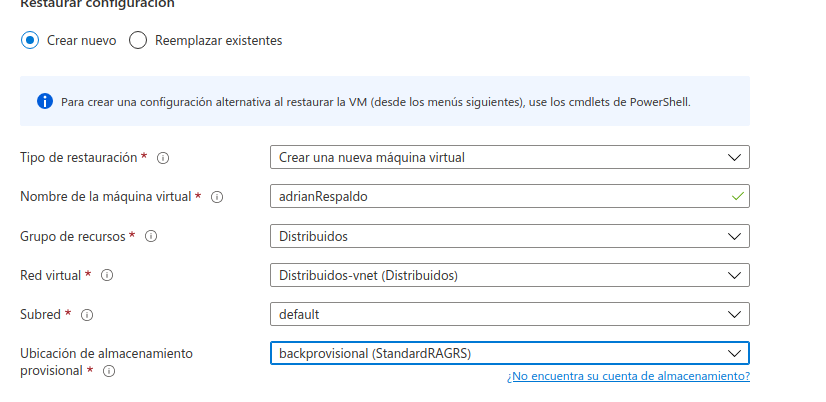
\includegraphics[scale=0.5]{imgs/12.png}\\
    \textit{Figura 14: Opciones a seleccionar posteriormente de la selección anterior}
    \fillandplacepagenumber
  \end{landscape}
  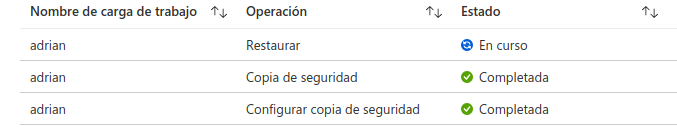
\includegraphics[scale=0.5]{imgs/13.png}\\
  \textit{Figura 15: En espera de completar la restauración}\\
  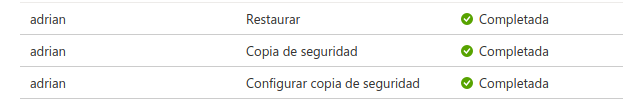
\includegraphics[scale=0.5]{imgs/14.png}\\
  \textit{Figura 16: Respaldo completado}
\end{center}
\begin{landscape}
  \subsection{Eliminación del proceso de respaldos}
  Por ultimo lo que haremos es lo siguiente:
  \begin{center}
    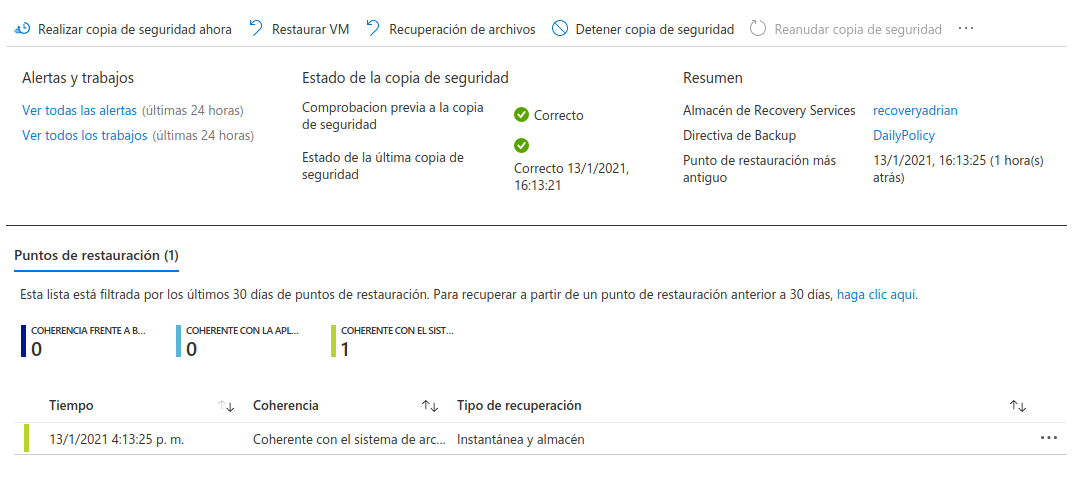
\includegraphics[scale=0.5]{imgs/15.png}\\
    \textit{Figura 17: En el mismo menú de backup dar click en Detener copia de seguridad}\\
    \fillandplacepagenumber
    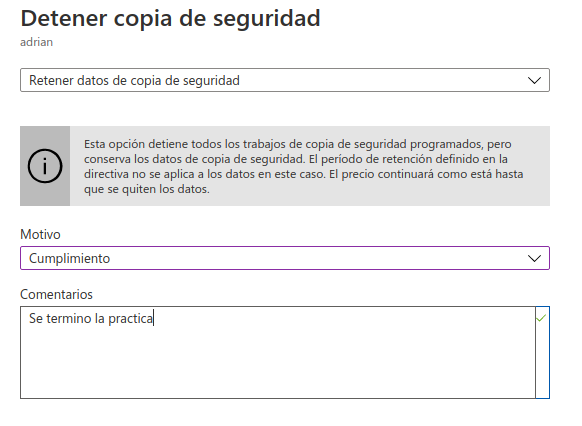
\includegraphics[scale=0.45]{imgs/16.png}\\
    \textit{Figura 18: Campos a llenar}\\
    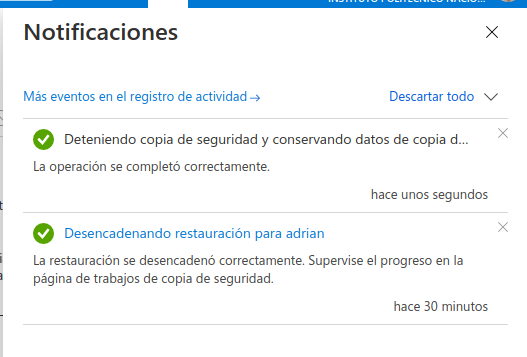
\includegraphics[scale=0.45]{imgs/17.png}\\
    \textit{Figura 19: Proceso completado}
  \end{center}
  \fillandplacepagenumber
  \clearpage
Finalmente ante completar todo esto, es necesario eliminar todos los recursos para evitar gastar el crédito gratuito de Azure.
\section{Conclusiones}
La realización de respaldos en una maquina en la nube es de mucha utilidad ya que nos permite pensar y darnos cuenta en como se puede llegar a migrar servidores completos de un lugar a otro sin necesidad de obtener de forma gratuita dolores de cabeza como el que ya no exista el empaquetado o el modulo en cierta distribución para correr cierto programa o cualquier otra problemática.

\end{landscape}

\end{document}
